% 2007 年湖北卷理科第 19 题：抛物线 x²=2py，C(0,p)，过 C 的直线交抛物线
%   于 A、B；N 为 C 关于原点的对称点（N(0,-p)）。
% 来源 PDF：gaokaomath-src/普通高考/2007/2007湖北理.pdf
% SHA-256：e767bc35f619e1cd5a96990bd14ba9415b3a440d7d9f5766e43aa6433844b65d
% 原页：2007湖北理.pdf 第 2 页（A3 三栏）第 1 栏，书页码 376。
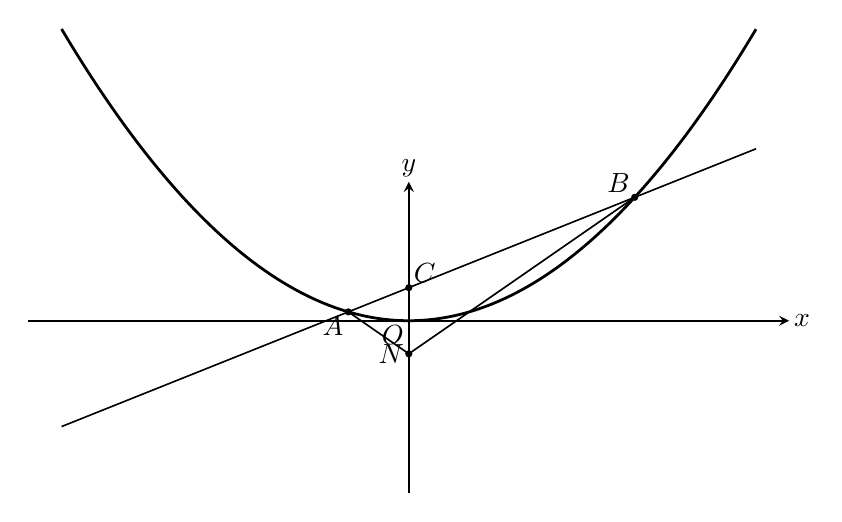
\begin{tikzpicture}[x=1.05cm, y=0.42cm, semithick,
  every node/.style={inner sep=1.5pt}]
  \draw[->,>=stealth] (-4.6,0) -- (4.6,0) node[right] {$x$};
  \draw[->,>=stealth] (0,-5.2) -- (0,4.2) node[above] {$y$};
  \node[below left] at (0,0) {$O$};

  % 抛物线 x^2=2py，取 p=1（示意图）
  \draw[line width=1pt, domain=-4.2:4.2, samples=100] plot ({\x},{\x*\x/2});

  % 过 C(0,1) 的直线
  \draw (-4.2,-3.2) -- (4.2,5.2);
  \coordinate (C) at (0,1);
  \fill (C) circle (1.3pt);
  \node[above right] at (C) {$C$};

  % A、B 交点（取直线 y=0.5x+1 与 x^2=2y）
  \coordinate (A) at (-0.732,0.268);
  \coordinate (B) at (2.732,3.732);
  \fill (A) circle (1.3pt);
  \fill (B) circle (1.3pt);
  \node[below left] at (A) {$A$};
  \node[above left] at (B) {$B$};

  % N 为 C 关于原点的对称点
  \coordinate (N) at (0,-1);
  \fill (N) circle (1.3pt);
  \node[left] at (N) {$N$};
  \draw (A) -- (N) -- (B);
\end{tikzpicture}
